\documentclass[11pt,a4paper]{scrartcl}

% Pakete
\usepackage[english]{babel}
\usepackage[UKenglish]{isodate}
\usepackage{xcolor}
\usepackage{graphicx}
\usepackage{amsmath}
\usepackage{amssymb}
\usepackage{nicefrac}
\usepackage[utf8]{inputenc}
\usepackage{siunitx}
\sisetup{
output-decimal-marker={.},
exponent-product=\cdot }
\usepackage{esvect}
\usepackage{eqnarray}
\usepackage{placeins}
\usepackage{scrpage2}
\usepackage{nameref}
\usepackage{upgreek}
\usepackage{caption}
\usepackage{subcaption}
\usepackage{bm}
\usepackage{mwe}
\usepackage{tcolorbox}
\usepackage{listings}
\usepackage{xstring}
\usepackage{stringstrings}
\usepackage{floatflt}
\usepackage{pgfplots}
\usepackage{tikz}
%\usepackage{physics}


% Custom colors
\definecolor{deepblue}{rgb}{0,0,0.5}
\definecolor{deepred}{rgb}{0.6,0,0}
\definecolor{deepgreen}{rgb}{0,0.5,0}
\DeclareFixedFont{\ttb}{T1}{txtt}{bx}{n}{12} % for bold
\DeclareFixedFont{\ttm}{T1}{txtt}{m}{n}{12}  % for normal

% tikz
\usetikzlibrary{arrows}

% caption setup
\captionsetup[subfigure]{labelformat=simple, labelsep=colon}
\renewcaptionname{english}{\figurename}{Fig.}
\renewcommand{\thesubfigure}{\arabic{figure}.\arabic{subfigure}}
\renewcommand{\thesubtable}{\arabic{table}.\arabic{subtable}}

% Listning Einstellungen
\lstloadlanguages{python}       % Default highlighting set to "python"
\DeclareCaptionFont{white}{\color{white}}
\DeclareCaptionFormat{listing}{%
  \parbox{0.99\textwidth}{\colorbox{gray}{\parbox{0.99\textwidth}{#1#2#3}}\vskip+5pt}}
\captionsetup[lstlisting]{format=listing, labelfont=white, textfont=white}
\lstset{frame=lrb,xleftmargin=\fboxsep,xrightmargin=-\fboxsep}
\pagestyle{empty}
\lstset{escapeinside={<@}{@>}}
\lstdefinestyle{MyPythonStyle}{
		language=Python,
		numbers=left,
		breaklines=true,
		basicstyle=\ttm,
		otherkeywords={self},             % Add keywords here
		keywordstyle=\ttb\color{deepblue},
		emph={MyClass,__init__},          % Custom highlighting
		emphstyle=\ttb\color{deepred},    % Custom highlighting style
		stringstyle=\color{deepgreen},
		frame=tb,                         % Any extra options here
		showstringspaces=false            % 
		}
\lstdefinestyle{MyCStyle}{
		language=C,
		numbers=left,
		tabsize=4,
		breaklines=true,
		basicstyle=\ttm,
		otherkeywords={self},             % Add keywords here
		keywordstyle=\ttb\color{deepblue},
		emph={MyClass,__init__},          % Custom highlighting
		emphstyle=\ttb\color{deepred},    % Custom highlighting style
		stringstyle=\color{deepgreen},
		frame=tb,                         % Any extra options here
		showstringspaces=false            % 
		}
\renewcommand{\lstlistingname}{Code block}
\renewcommand{\lstlistlistingname}{List of \lstlistingname s}

% Griechische Buchstaben vereinheitlichen
\renewcommand{\alpha}{\upalpha}
\renewcommand{\beta}{\upbeta}
\renewcommand{\gamma}{\upgamma}
\renewcommand{\delta}{\updelta}
\newcommand{\w}{\omega}
\newcommand{\la}{\lambda}

% Eigene mathematische Kommandos
\newcommand{\dd}{\text{d}} 							% Differential
\newcommand{\p}{\partial} 								% Partielles Differential
\newcommand{\D}{\Delta} 								% Fehler / Laplace
\newcommand{\order}[1]{\math\newpage
cal{O}\left( #1 \right)}
\newcommand{\abs}[1]{\left| #1\right|} 					% Betrag
\newcommand{\Max}[1]{\max \left\lbrace #1\right\rbrace} % max{}
\newcommand{\Min}[1]{\min \left\lbrace #1\right\rbrace} % min{}
\newcommand{\diff}[2]{\frac{\text{d} #1}{\text{d} #2}}	% Ableitung
\newcommand{\pdiff}[2]{\frac{\partial #1}{\partial #2}} % Partielle Ableitung
\newcommand{\errprop}[2]{\left| \frac{\partial #1}{\partial #2}\right| \cdot \Delta #2}

% Klammern
\newcommand{\lk}{\left\langle}
\newcommand{\rk}{\right\rangle}
\newcommand{\lb}{\left\lbrace}
\newcommand{\rb}{\right\rbrace}
\newcommand{\lc}{\left(}
\newcommand{\rc}{\right)}
												% Fehlerfortpflanzung
\newcommand{\rel}[1]{\frac{\Delta #1}{#1}}				% Relativer Fehler

% Eigene trigonometrische Funktionen
\newcommand{\Exp}[1]{\text{exp}\left( #1 \right)}		% exp()
\newcommand{\Ln}[1]{\text{ln}\left( #1 \right)}			% ln()
\newcommand{\Log}[1]{\text{log}\left( #1 \right)}		% log()
\newcommand{\Sin}[1]{\text{sin}\left( #1 \right)}     	% sin()
\newcommand{\Cos}[1]{\text{cos}\left( #1 \right)}		% cos()
\newcommand{\Sinz}[1]{\text{sin}^2\left( #1 \right)}	% sin^2()
\newcommand{\Cosz}[1]{\text{cos}^2\left( #1 \right)}	% cos^2()
\newcommand{\Tan}[1]{\text{tan}\left( #1 \right)}		% tan()
\newcommand{\Asin}[1]{\text{asin}\left( #1 \right)}		% asin()
\newcommand{\Acos}[1]{\text{acos}\left( #1 \right)}		% acos()
\newcommand{\Atan}[1]{\text{at\newpage
an} \left( #1 \right)}	% atan()

% Eigene Vektor Kommandos
\newcommand{\tovec}[2]{\begin{pmatrix}#1\\ #2\end{pmatrix}}	% 2D-Vektor
\newcommand{\trvec}[3]{\begin{pmatrix}#1\\ #2\\ #3\end{pmatrix}}	% 3D-Vektor	
\newcommand{\ovec}[1]{\boldsymbol{#1}}

% Eigene Referenz-Kommandos
\newcommand{\eref}[1]{(\ref{#1})}						% Gleichungen
\newcommand{\sref}[2]{\subref{#2}}						% Unterabbildungen
\newcommand{\kref}[1]{\ref{#1} \glqq\nameref{#1}\grqq}  % Kapitel
\newcommand{\lref}[1]{$[#1]$}							% Quellen: \newcommand{\lit}{1} => \lref{\lit}

% listing commandos
\newcommand{\listfile}[7][MyPythonStyle]{
\lstinputlisting[linerange={#4-#5}, firstnumber=#4, caption={#6} \hfill script:  #3, label=#7, style=#1]{#2}}
% arguments:
% \listfile[style]{location/filename}{filename}{firstline}{lastline}{title}{label}
% Imports code from a file 
% You will have to escape the filename and the title
% style is an optional argument.

\newcommand{\ls}[1]{\lstinline@#1@}

% using \lstinline@code@ for code in line
% works with every sign instead of @

% commands for this task
\newcommand{\ua}{AU}
\newcommand{\vecx}[1]{\ovec{x}^{(#1)}}
\newcommand{\vecv}[1]{\ovec{v}^{(#1)}}
\newcommand{\veca}[1]{\ovec{a}^{(#1)}}
\newcommand{\vecF}[1]{\ovec{F}^{(#1)}}
\newcommand{\vecr}[1]{\ovec{r}^{(#1)}}
\newcommand{\nx}[1]{x^{(#1)}}
\newcommand{\nv}[1]{v^{(#1)}}
\newcommand{\na}[1]{a^{(#1)}}
\newcommand{\nm}[1]{m^{(#1)}}
\newcommand{\nF}[1]{F^{(#1)}}
\newcommand{\nr}[1]{r^{(#1)}}
\newcommand{\Ekin}{E_\text{kin}}
\newcommand{\Ekino}{E_{\text{kin},0}}
\newcommand{\fr}{f_\text{re}}
\newcommand{\fij}{\ovec{f}_{ij}}
\newcommand{\rij}{\ovec{r}_{ij}}
\newcommand{\fji}{\ovec{f}_{ji}}
\newcommand{\rji}{\ovec{r}_{ji}}
\newcommand{\rj}{\ovec{r}_{j}}
\newcommand{\ri}{\ovec{r}_{i}}



% Kopf-/Fusszeile
\pagestyle{scrheadings}
\clearscrheadfoot
\chead{Simulation Methods in Physics I}
\ihead{Worksheet 3}
\ohead{\today}
\ofoot{\pagemark}
\ifoot{Michael Marquardt, Cameron Stewart}

\begin{document}

% Titelseite
\begin{titlepage}

\ \\ \ \\ \ \\

\center\textbf{
\begin{large}
Simulation Methods in Physics I
\end{large} \\ \ \\
\begin{Large}
Worksheet 5: Monte-Carlo
\end{Large}}   \\ \ \\
\ \\ \ \\

\begin{tabular}{lll}
Students: &Michael Marquardt &Cameron Stewart\\ 
matriculation numbers: &3122118 &3216338\\
\end{tabular}

\end{titlepage}

% Inhaltsverzeichnis

% -------------------------------------- Begin Of Document ----------------------------------------

\section{Simple Sampling - Integration}
In this worksheet we will use the Monte Carlo technique to integrate a function and to look at the Ising 
spin model. The Monte Carlo method is a statistical technique for computing expectation values that are 
given by
\begin{equation}
\langle A \rangle = \frac{\int_\Phi A(\phi) P(\phi) d\phi}{\int P(\phi) d\phi}
\label{eq:exp}
\end{equation}
where $A$ is an observable, $P$ is the probability of finding the system in a certain state, $\phi$ is a state of the system and $\Phi$ is the set of all states of the system.

The Monte Carlo simply replaces these integrals with finite sums over random states of the system as
\begin{equation}
\langle A \rangle = \frac{\sum_N A(\phi) P(\phi) d\phi}{\sum_N P(\phi) d\phi}.
\label{eq:mc}
\end{equation}
If the states $\phi$ are randomly distributed then this is called simple sampling.

We can use the Monte Carlo method to evaluate an integral if we set $\phi = x$ and let $P(x)$ be constant. Equate eqs. \ref{eq:exp} and \ref{eq:mc} and solve for the integral leaves us with
\begin{equation}
\int_a^b f(x) dx = \frac{b-a}{N} \sum_N f(x_i)
\label{eq:int}
\end{equation}
where we have renamed $A$ to $f$.

We begin this worksheet by using this method to evaluate the integral of the Runge function over the interval $[-5, 5]$. The Runge function is given by
\begin{equation}
f(x) = \frac{1}{1+x^2}
\end{equation}
and its integral is 
\begin{equation}
\int_a^b \frac{1}{1+x^2} dx = \arctan(b)-\arctan(a).
\end{equation}

We begin by writing a simple function in python to compute the Runge function and another to compute its integral.
\listfile{../src/mon_car.py}{src/mon\_car.py}{3}{7}{Runge Function}{runge}
\begin{figure}[ht]
	\centering
	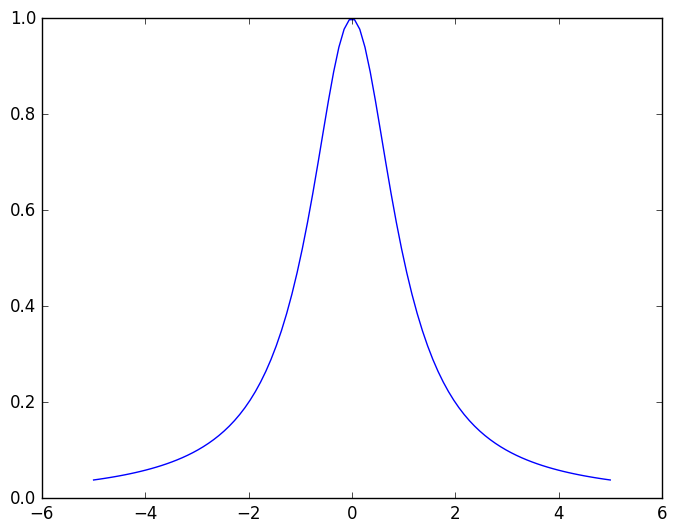
\includegraphics[width=0.7\textwidth]{../fig/rungeplot.png}
	\caption{Plot of the Runge function from $-5$ to $5$.	}
	\label{fig:runge}
\end{figure}
The Runge function is plotted in fig. \ref{fig:runge}

Now we will use a simple sampling Monte Carlo technique to evaluate the integral. Equation \ref{eq:int} is implemented as:
\listfile{../src/mon_car.py}{src/mon\_car.py}{9}{12}{Simple Sampling}{simple}
This allows us to set a function, upper and lower bound, and number of samples as parameters. The measured value of the integral and the standard error of the mean are returned. 

We now write a program to use our Monte Carlo algorithm to compute this integral for a number of samples $N = 2^i$ with $2 \leq i \leq 20$. 
\listfile{../src/integration.py}{src/integration.py}{5}{13}{Simple Sampling}{simpsamp}
\begin{figure}[ht]
	\centering
	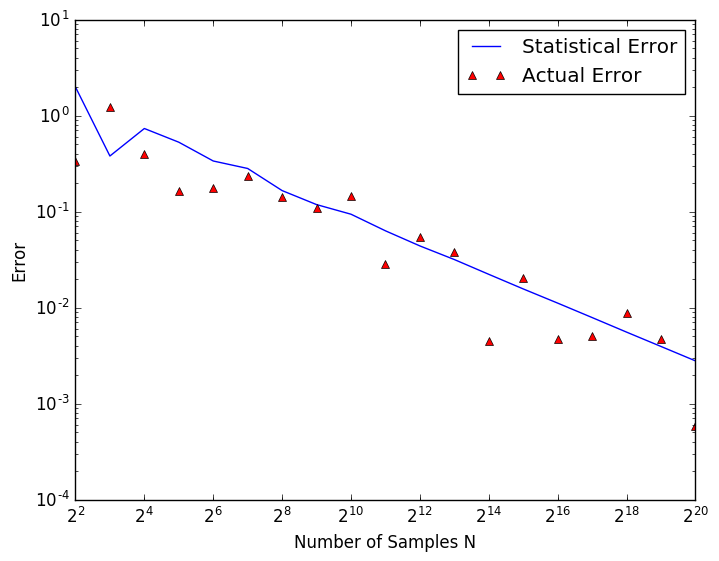
\includegraphics[width=0.7\textwidth]{../fig/simple_err.png}
	\caption{Plot of the statistical vs actual error in our simple sampling evaluation of the integral of the Runge function for various number of samples.	}
	\label{fig:simple}
\end{figure}
Figure \ref{fig:simple} shows the statistical vs. actual error in our calculation of this integral for our range of samples. We used a log-log plot for readability.

\section{Importance Sampling}

\subsection{Implementation}

The goal of this task is to implement the Metropolis-Hastings algorithm, which generates states $\Phi_i$ form a given probability-distribution $P(\Phi_i)$ instead of weight the observable $A(\Phi_i)$ with $P(\Phi_i)$ like it is the case for the simple sampling method.
This algorithm is implemented in the file \lstinline|metropolis.py|.

\listfile{../src/metropolis.py}{src/metropolis.py}{3}{16}{Metropolis algorithm}{metro}

In order to do this the algorithm generates a new state$\Phi_{i+1}$ from the old state $\Phi_i$ via a function \lstinline@trial_move()@ in line 10.
Thereby the new state must be random in some way.
Then in the if/else-statement the new state is accepted with an probability $\Min{1,P(\Phi_{i+1})/P(\Phi_i)}$.\\

At the end the function returns a list of N+1 states and the acceptance rate $\alpha$.

\subsection{Use Metropolis for Runge Function}

Now the Metropolis algorithm should be used to generate $N=100 ,000$ samples of an scalar state $\Phi =x$ which should be distributed according to the Runge function.
Therefor the trial move should be an uniform random number in the interval $[x-\D x, x+\D x]$ with $\D x\in \lb 0.1, 1, 10, 100\rb$.\\

The trial move is implemented in \lstinline|metropolis.py|.

\listfile{../src/metropolis.py}{src/metropolis.py}{18}{23}{Trial move}{tm}

As you can see there is another function \lstinline|trial_move_set_dx| which is used to set the global variable \lstinline|tm_dx|.\\

The main loop is implemented in \lstinline@imp_samp.py@.

\listfile{../src/imp_samp.py}{src/imp\_samp.py}{12}{24}{Importance sampling}{impsamp}

In lines 7-11 the necessary variables are initialized.
You can set the initial state $x_0$ by passing \ls{--x0 <value>} when call the function. Its default value is a random number in between $-5$ and $5$.
The main for loop sets \ls{tm_dx} to $\D x$ and runs the metropolis() function for the different $\D x$.\\

As probability-distribution the function \ls{runge()} is used. 
Because of only using it in a fraction $P(\Phi_{i+1})/P(\Phi_i)$ the function must not be normalized.

\subsection{Evaluation}

\begin{figure}[ht]
	\centering
	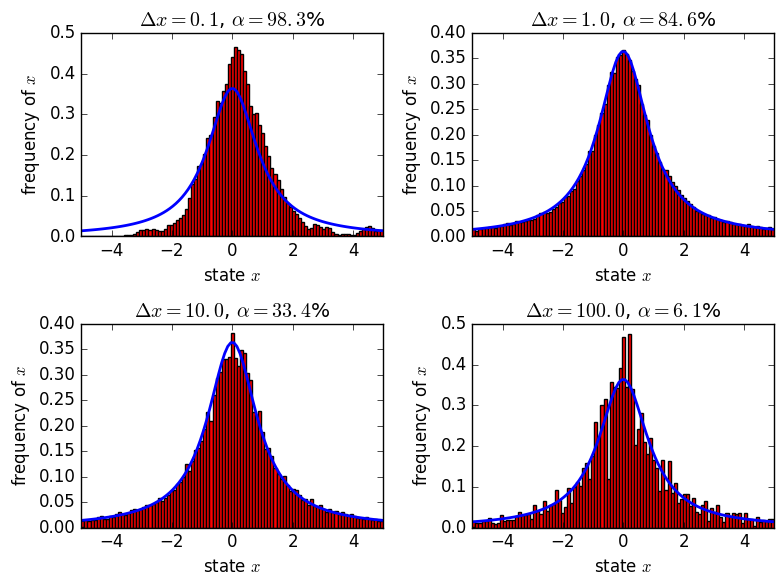
\includegraphics[width=1\textwidth]{../fig/metroplot.png}
	\caption{
		Histogram of the frequency of the states $x$ generated by the Metropolis algorithm in red.
		The blue curve is the normalized Runge function.}
	\label{metroplot}
\end{figure}

The results of the Metropolis algorithm for an initial state $x_0=0$ are shown in figure \ref{metroplot}.
This initial value is chosen because it is the most likely state.\\

As you can see steps of $\D x=0.1$ lead us to no useful distribution. 
For example values below $x=-4$ are not generated at all, what shows that the change of the state in one step is to small.
For some other tries and initial values it became even worse.
Therefore $\D x=0.1$ is to small.\\

Both $\D x=1$ and $\D x=10$ produce good distributions, but $\D x=1$ is a little better than $\D x=10$.\\

The many small peaks in the distribution for $\D x=100$ show that $\D x=100$ is to high.
The peaks come from values which did not change for a longer period because the probability to accept the new state was too low.\\

When taking a look at the acceptance rate $\alpha$ you can see that it decreases with increasing $\D x$.\\

For $\D x=0.1$ the acceptance rate is nearly $\SI{100}{\percent}$. 
This means the resulting algorithm is more or less a random walk with no respect to the given probability distribution.\\

The best result is measured for $\D x=1$ with $\alpha =\SI{84.6}{\percent}$, but also $\D x=10$ with only $\alpha =\SI{33.4}{\percent}$ produces good distributions.
Therefore it may be good to kepp the acceptance rate between $\SI{35}{\percent}$ and $\SI{85}{\percent}$.\\

$\D x=100$ produces a acceptance rate of only $\alpha =\SI{6.1}{\percent}$. 
The effects are mentioned above.

\FloatBarrier
\section{Simulating the Ising Model}
Now we will look to simulate the two dimensional Ising spin model on an $(L \times L)$ square lattice.	The total energy of the system is 
\begin{equation}
\frac{1}{2}\sum_{i=0}^{L-1}\sum_{j=0}^{L-1}E_{i,j}
\end{equation}
with
\begin{equation}
E_{i,j} = -\sigma_{i,j}(\sigma_{i+1,j} + \sigma_{i-1,j} + \sigma_{i,j+1} + \sigma_{i,j-1}).
\end{equation}
Spins can take the values $\pm 1$ and we use periodic boundary conditions.

The observables we are interested in are the energy density
\begin{equation}
e =\left \langle \frac{E}{L^2}\right\rangle
\end{equation}
and the magnetization density
\begin{equation}
m = \langle |\mu| \rangle
\end{equation}
\begin{equation}
\mu = \frac{1}{L^2} \sum_{i=0}^{L-1}\sum_{j=0}^{L-1}\sigma_{i,j}
\end{equation}

The measurement of the total energy $E$ and magnetization density $\langle\mu\rangle$ for a given state are implemented as
\listfile{../src/ising_lib.py}{src/ising\_lib.py}{16}{31}{Observable Measurement}{observe}
\subsection{Exact Summation}
We begin by computing the expectation values of these two observables directly from the partition function. This is possible if we use a box size of $L=4$ which we will use for the rest of the worksheet. Expectation values of observables can be calculated by
\begin{equation}
\left\langle A \right\rangle = \frac{\sum_\Phi A_\phi e^{-E_\phi /T}}{\sum_\Phi e^{-E_\phi /T}}.
\label{eq:part}
\end{equation}
In order to calculate this sum we need to generate every possible state of the finite 2D Ising system. We do this by counting to $2^{16}$ in binary. All the necessary states are represented by all of the 16 digit binary numbers. We simply replace $0$ with $-1$ and map back onto a square lattice. The following function performs the neccesary generation.
\listfile{../src/ising_lib.py}{src/ising\_lib.py}{44}{56}{State Generation}{states}

Equipped with the set of states, we are prepared to calculate the sum in \ref{eq:part} for various temperatures $T = {1.0, 1.1, ..., 4.9, 5.0}$. This is accomplished for our observables of interest with the next code block.
\listfile{../src/ising_exact.py}{src/ising\_exact.py}{6}{16}{Exact Summation}{exact}

The blue curve in figures \ref{fig:ising_e} and \ref{fig:ising_m} show the expectaion values of our two observables due to exact summation.
\subsection{Monte Carlo}
The exact calculation in the preceding section is quite slow and will not withstand a simulation with more spins so we will use Monte Carlo simulation to obtain the same information. We will use the Metropolis-Hastings algorithm to select states. One Monte Carlo step is implemented as follows.
\listfile{../src/ising_lib.py}{src/ising\_lib.py}{33}{42}{Monte Carlo Step}{isingmc}
We then run $10000$ MC steps for each of our previously listed temperatures.
\listfile{../src/ising_mc.py}{src/ising\_mc.py}{5}{15}{MC Simulation}{isingmcdat}
The points in figures \ref{fig:ising_e} and \ref{fig:ising_m} show the values of magnetization and energy density measured via Monte Carlo.
\subsection{Error Analysis}
Since each step in our simulation is derived from the previous one, the data is obviously correlated and we can't use the obvious method for estimating error. In this case we will use binning analysis. This involves breaking our time series into $N_B$ bins. If the bin length $k$ is large enough then these bins will be uncorrelated. Clearly $\bar{O}_B = \bar{O}$ and we can calculate the squared error as
\begin{equation}
\epsilon^2_{\bar{O}} = \frac{1}{N_B(N_B-1))}\sum_{n=1}^{N_B}(O_{B,n} - \bar{O})^2,
\end{equation}
correlation time as
\begin{equation}
\tau = \frac{k \epsilon^2_{\bar{O}}}{2 N \sigma^2_{O_i}},
\end{equation}
and effective sample size as 
\begin{equation}
N_{\mathrm{eff}} = N/2\tau
\end{equation}
In order to take care of the free parameter k, we perform the entire error analysis with $1 \leq k \leq N/10$ and take the highest autocorrelation time.
\listfile{../src/ising_lib.py}{src/ising\_lib.py}{65}{93}{Error Analysis}{error}

In order to test our error analysis we will calculate statistics about a bivariate Gaussian. We use the following function to generate samples from a bivariate Gaussian.
\listfile{../src/ising_lib.py}{src/ising\_lib.py}{58}{63}{Bivariate Gaussian}{gauss}
We choose $N = 1e6$ and $\rho = 0.99005$ and the autocorrelation time is known to be
\begin{equation}
\tau = \frac{1}{2}\frac{1+\rho}{1-\rho} \approx 100.003
\end{equation}
Using our error\_analysis function we find
\begin{equation}
\bar{O}=-0.0054, \quad k = 15625, \quad \tau = 104.2, \quad N_\mathrm{eff} = 4699.6, \quad \epsilon^2_{\bar{O}} = 0.0143
\end{equation}
Finally we use our analysis program to calculate the error in the MC measurements of energy and magnetization density.
\begin{figure}[ht]
	\centering
	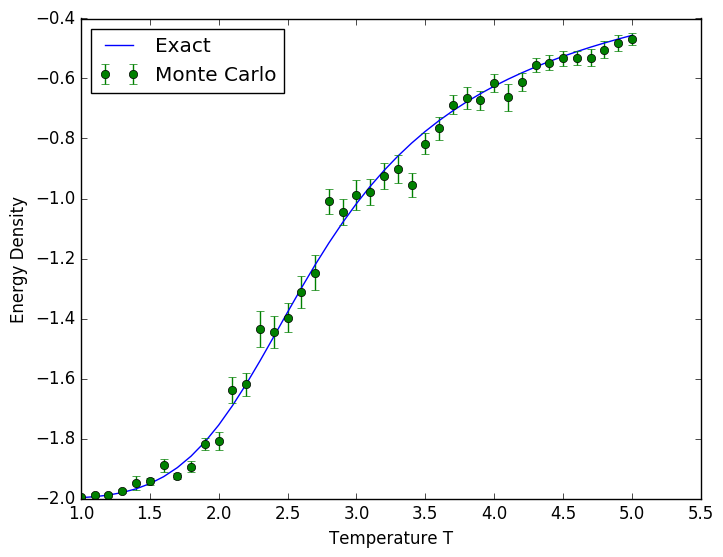
\includegraphics[width=0.7\textwidth]{../fig/errorplot_e.png}
	\caption{
		Energy density of our 2D Ising spin system as a function of temperature. The blue curve is due to exact summation and the points refer to the Monte Carlo algorithm. Error bars are calculated using binning analysis.}
	\label{fig:ising_e}
\end{figure}
\begin{figure}[ht]
	\centering
	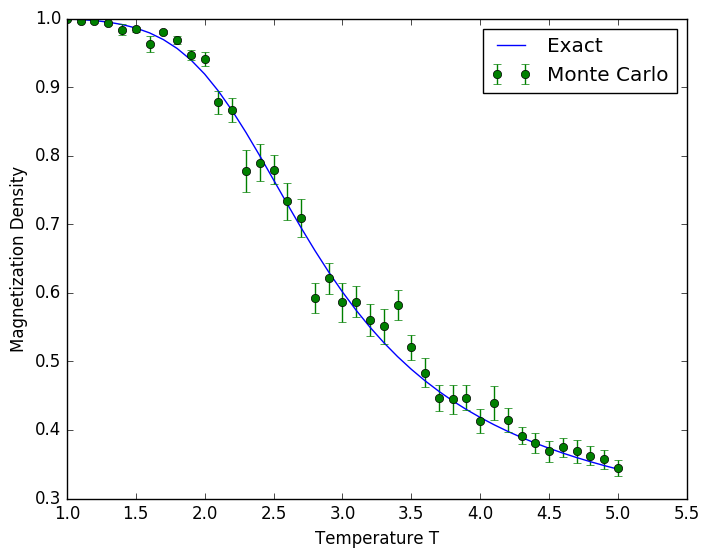
\includegraphics[width=0.7\textwidth]{../fig/errorplot_m.png}
	\caption{
		Magnetization density of our 2D Ising spin system as a function of temperature. The blue curve is due to exact summation and the points refer to the Monte Carlo algorithm. Error bars are calculated using binning analysis.}
	\label{fig:ising_m}
\end{figure}

\end{document}

